\documentclass[xcolor=svgnames]{beamer}
%\usetheme{Rochester}
\usetheme{Madrid}


\usepackage{multimedia}
\usepackage{cite}
\usepackage{float}
\usepackage{ulem}
\usepackage{listings}
\lstset{language=Python, basicstyle=\scriptsize}
\usepackage{verbatim}

\usepackage{graphicx}
\definecolor{titlecolor}{HTML}{F6CD03}%{FFD82F}  % e.g. for block title
\definecolor{titlefill}{HTML}{333367}%{006900}  % e.g. for block title
\usecolortheme[rgb={0.2,0.2,0.40392}]{structure}%rgb={0.0,0.5,0.0}
\setbeamercolor{frametitle}{bg=titlefill,fg=titlecolor}
\setbeamercolor{normal text}{fg=black}
\setbeamercolor{lower separation line head}{bg=black}
\setbeamercolor{title}{bg=titlefill,fg=titlecolor}
\setbeamercolor{block title}{fg=titlecolor}
%%\setbeamertemplate{navigation symbols}{}
\setbeamertemplate{items}[triangle]

\setbeamertemplate{footline}{
  \begin{beamercolorbox}[wd=\paperwidth,ht=0.25cm,center]
    {section in head/foot}
    \begin{beamercolorbox}[wd=0.9\paperwidth,ht=0.25cm,center]
      {section in head/foot}
      \raisebox{0.05cm}{Python Programming}
    \end{beamercolorbox}
    \begin{beamercolorbox}[wd=0.09\paperwidth,ht=0.25cm,right]
      {section in head/foot}
      \raisebox{0.05cm}{\insertframenumber}
    \end{beamercolorbox}
  \end{beamercolorbox}
}




\definecolor{mygreen}{rgb}{0,0.6,0}
\definecolor{mygray}{rgb}{0.95,0.95,0.95}
\definecolor{mygraybl}{rgb}{0.95,0.95,0.995}
\definecolor{mymauve}{rgb}{0.58,0,0.82}
\definecolor{mypink}{rgb}{0.99,0.86,0.95}


\lstnewenvironment{code}
{\lstset{frame=single, basicstyle=\footnotesize\ttfamily, backgroundcolor=\color{mygray},
columns=fullflexible }}
{\vspace*{-9pt}}

\lstnewenvironment{codeout}
{\lstset{frame=none, basicstyle=\footnotesize\ttfamily, backgroundcolor=\color{mygraybl},
columns=fullflexible }}
{\vspace*{-2pt}}

\lstnewenvironment{errout}
{\lstset{frame=none, basicstyle=\footnotesize\ttfamily, backgroundcolor=\color{mypink},
columns=fullflexible }}
{\vspace*{-2pt}}

\lstnewenvironment{editor}
{\lstset{frame=tb, basicstyle=\footnotesize\ttfamily, columns=fullflexible}}
{\vspace*{-9pt}}

\lstnewenvironment{terminal}
{\lstset{frame=l, basicstyle=\footnotesize\ttfamily, columns=fullflexible}}
{\vspace*{-9pt}}


\newenvironment{userin}
{\vspace*{-6pt} User: \itshape }
{\vspace*{-2pt}\normalfont  }

\title{Tala - Distributed Computing}
\author{Jeff McGough}
\institute{Department of Computer Science and Engineering\\
  South Dakota School of Mines and Technology\\
  Rapid City, SD 57701, USA}

\date{\today}

\begin{document}

%----------- titlepage ----------------------------------------------%
\begin{frame}[fragile]
\titlepage

\end{frame}




%----------- slide --------------------------------------------------%
\section[Tala]{Tala}
\begin{frame}[fragile]
  \frametitle{Tala}
\begin{Large}
Tala \\[5mm]
Distributed Communications
\end{Large}
\end{frame}





%----------- slide --------------------------------------------------%

\begin{frame}[fragile]
  \frametitle{Problem}

What if you want to send a message between two processes:
\begin{center}
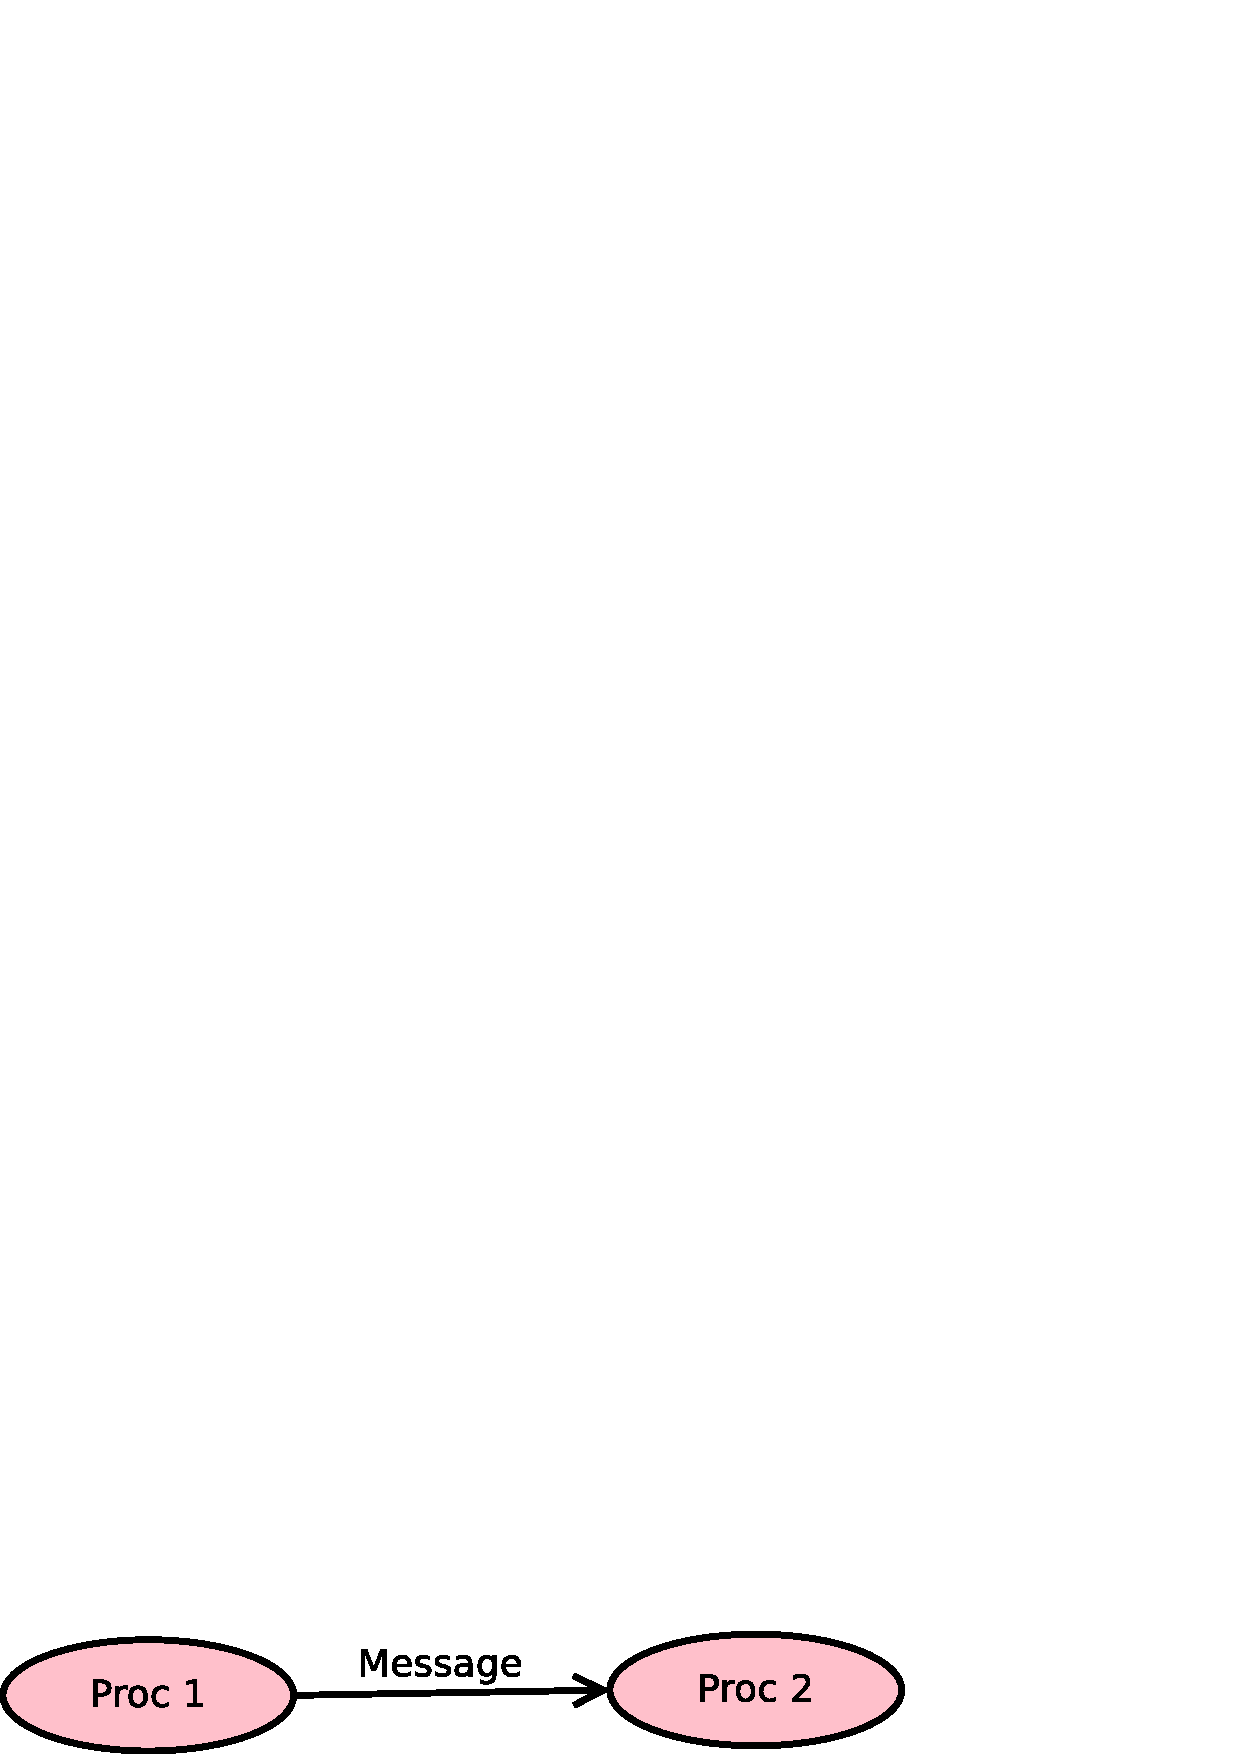
\includegraphics[width=7cm]{./Image1.pdf}
\end{center}
There are a lot of approaches to this problem.  File system (files and pipes)
are easy, but not efficient. For processes on different
address spaces, using shared memory does not work.  And neither files or SHM will
work on when using completely separate systems.  

\vfill
Using sockets is the popular answer.

\end{frame}


%----------- slide --------------------------------------------------%

\begin{frame}[fragile]
\frametitle{Sockets}
  
There are several issues using sockets
\begin{itemize}
\item You need to know the location of the process. IP address and Port
must be known.  
\item There must be some synchronization, buffering or queuing between the processes.
\item Your communication pattern needs to be client server where the 
sending process is the client and receiving process is the server. 
It is asymmetrical in nature.
\item Socket libraries support low level communications and not the communication 
patterns we would like such as Publish/Subscribe.
\item In all but the most simple applications, it requires a threaded design.
\end{itemize} 

\end{frame}



%----------- slide --------------------------------------------------%

\begin{frame}[fragile]
\frametitle{Communication Patterns}

There are two patterns we will start with:
\begin{itemize}
\item Request - Reply : ReqRep
\item Publish - Subscribe :  PubSub
\end{itemize}\vfill

There are other patterns but for getting started on this project
these two will suffice.

\end{frame}


%----------- slide --------------------------------------------------%

\begin{frame}[fragile]
\frametitle{REQREP}


Request-Reply is a more traditional client server communication 
pattern. \vfill 

It is  one to one direct communication.
\vfill 
\begin{center}
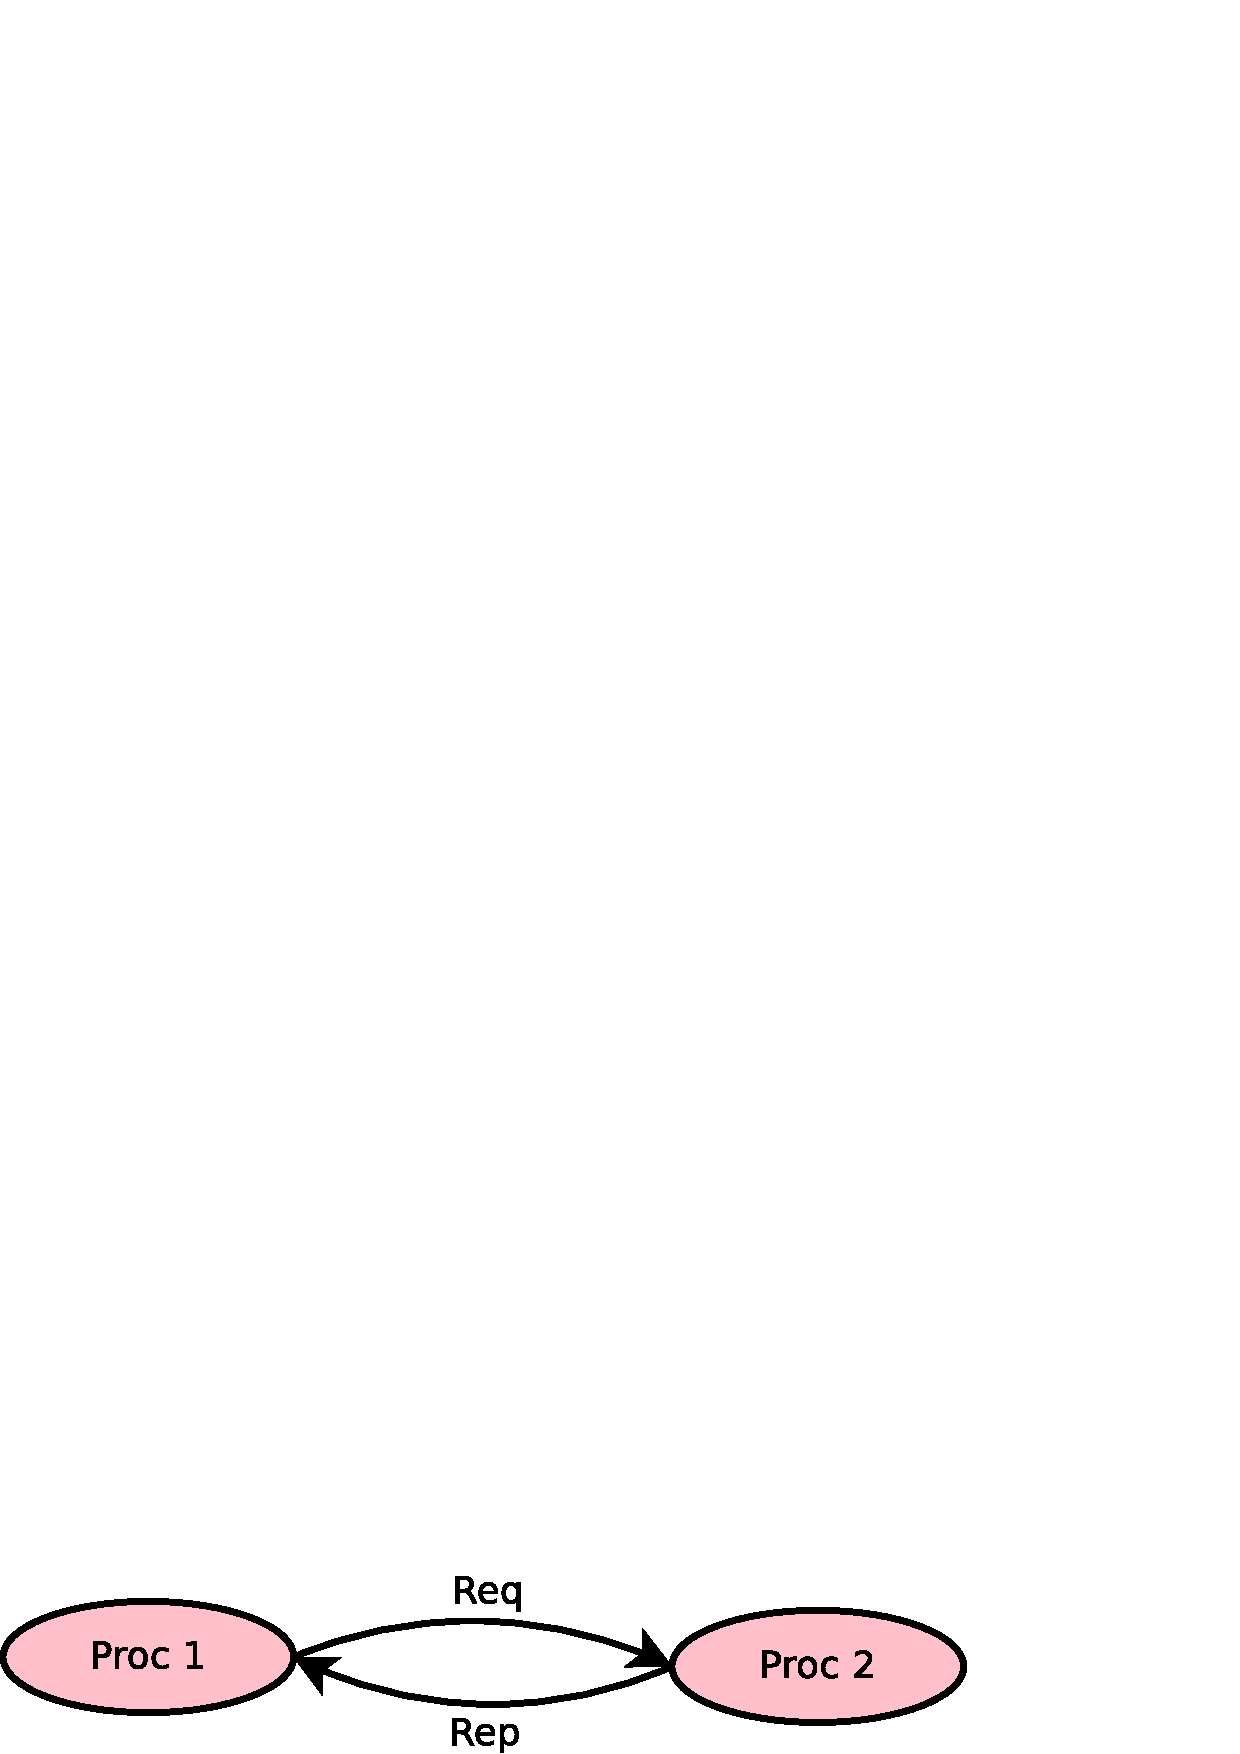
\includegraphics[width=7cm]{./Image2.pdf}
\end{center}
\vfill
 A client will send a message to the server requesting 
some information.  That is returned in the reply.   It is a client
initiated exchange.\vfill

This will be useful for one-off types of communication.

\end{frame}


%----------- slide --------------------------------------------------%

\begin{frame}[fragile]
\frametitle{PUBSUB}

Publish-Subscribe is our main communication pattern for this project.\vfill

Formally, it is a buffered, indirect, many to many communication pattern.\vfill

In PubSub, a process will {\it publish} a message on a named channel or \textit{topic}. This means that the 
message is placed in a message queue which is normally a FIFO. \vfill

\vfill 
\begin{center}
\includegraphics[width=9cm]{./Image3.pdf}
\end{center}
\vfill
A process that is subscribed
can receive the message off of the other end of the topic (FIFO).  Where this FIFO
is actually located is to be determined.
\end{frame}


%----------- slide --------------------------------------------------%

\begin{frame}[fragile]
\frametitle{PUBSUB}


  Any number of
processes can publish on the topic.   These messages are queued up in the  FIFO.
  
\vfill 
\begin{center}
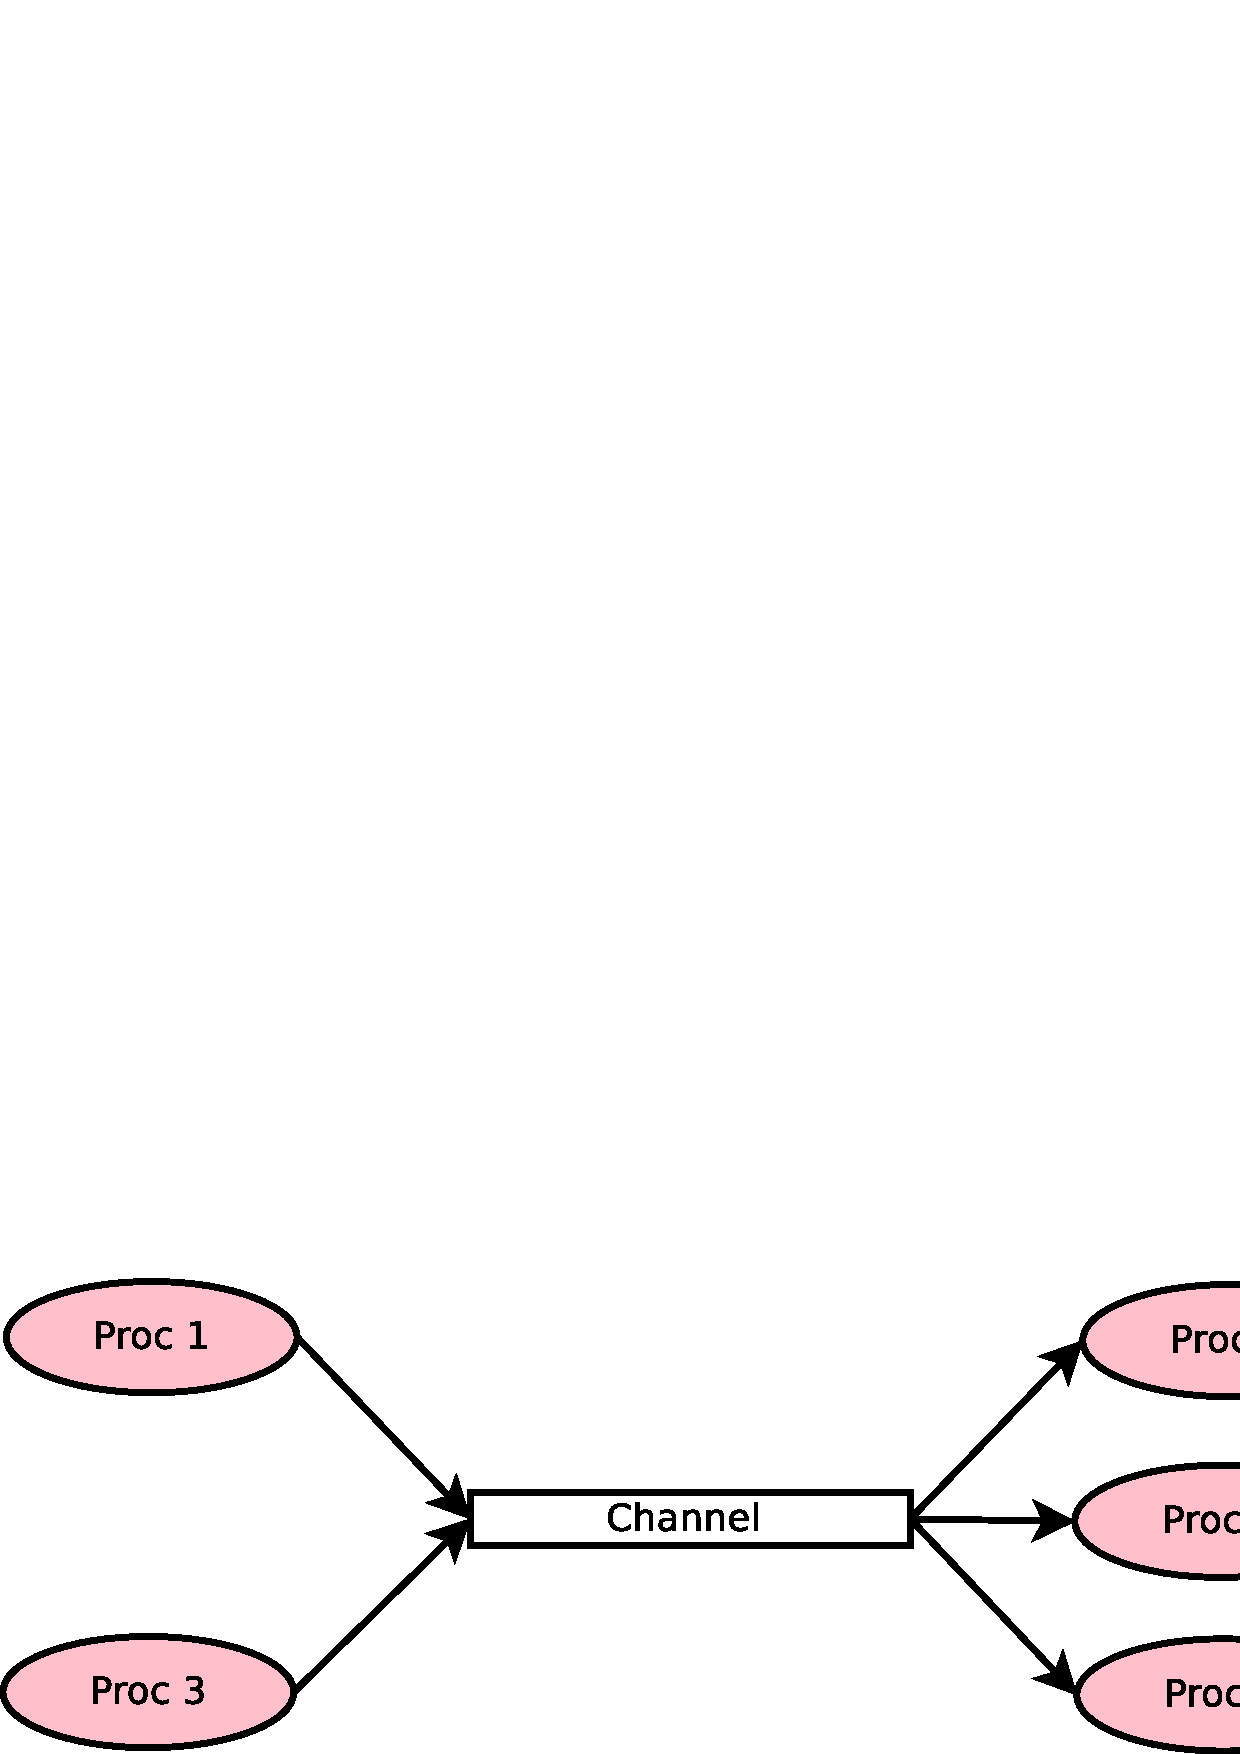
\includegraphics[width=9cm]{./Image4.pdf}
\end{center}

\vfill

Any number of processes may subscribe to the topic.  
\end{frame}



%----------- slide --------------------------------------------------%

\begin{frame}[fragile]
\frametitle{More details}

I should not need to know where my other processes are running. 
\vfill

I should only need to publish to a topic or subscribe
to a topic;.

\vfill

Topics can carry multiple messages and have a message type associated with them.
 
 
 
\end{frame}

%----------- slide --------------------------------------------------%

\begin{frame}[fragile]
\frametitle{Tala}

\begin{huge}
Tala
\end{huge}
\vfill

A fast distributed message system for remote interprocess communication.
 
\end{frame}

%----------- slide --------------------------------------------------%

\begin{frame}[fragile]
\frametitle{Usage}

The following graphical user story describes a common use case.
\vfill

Although not all aspects of Tala are represented here, this use case 
is essential to understand before moving on.
 
 \vfill
 
 In this example, we look at a design that has the FIFO or topic as a 
 standalone or separate entity.  The reasoning is that if the FIFO is 
 bound to either publisher or subscriber, it might limit the number of 
 publishers or subscribers (this will get us started for now).
 \vfill
 This is a design decision.  The following ``User Stories'' are to give
 a flavor of how the tool is used.  How the directory service is constructed
 or the details on communication topics are not defined.
 
\end{frame}

%----------- slide --------------------------------------------------%
\begin{frame}[fragile]
  \frametitle{User Story}
  
 Request to connect to a specific topic.   This can be built into a ``topic open" type function call.   Master process described later.
\begin{center}
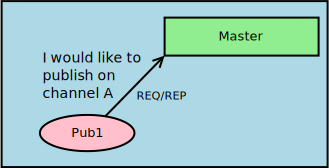
\includegraphics[width=9cm]{./Diagram1.pdf}
\end{center}
\end{frame}


%----------- slide --------------------------------------------------%
\begin{frame}[fragile]
  \frametitle{User Story}
First time, the topic does not exist and needs to be created.
\begin{center}
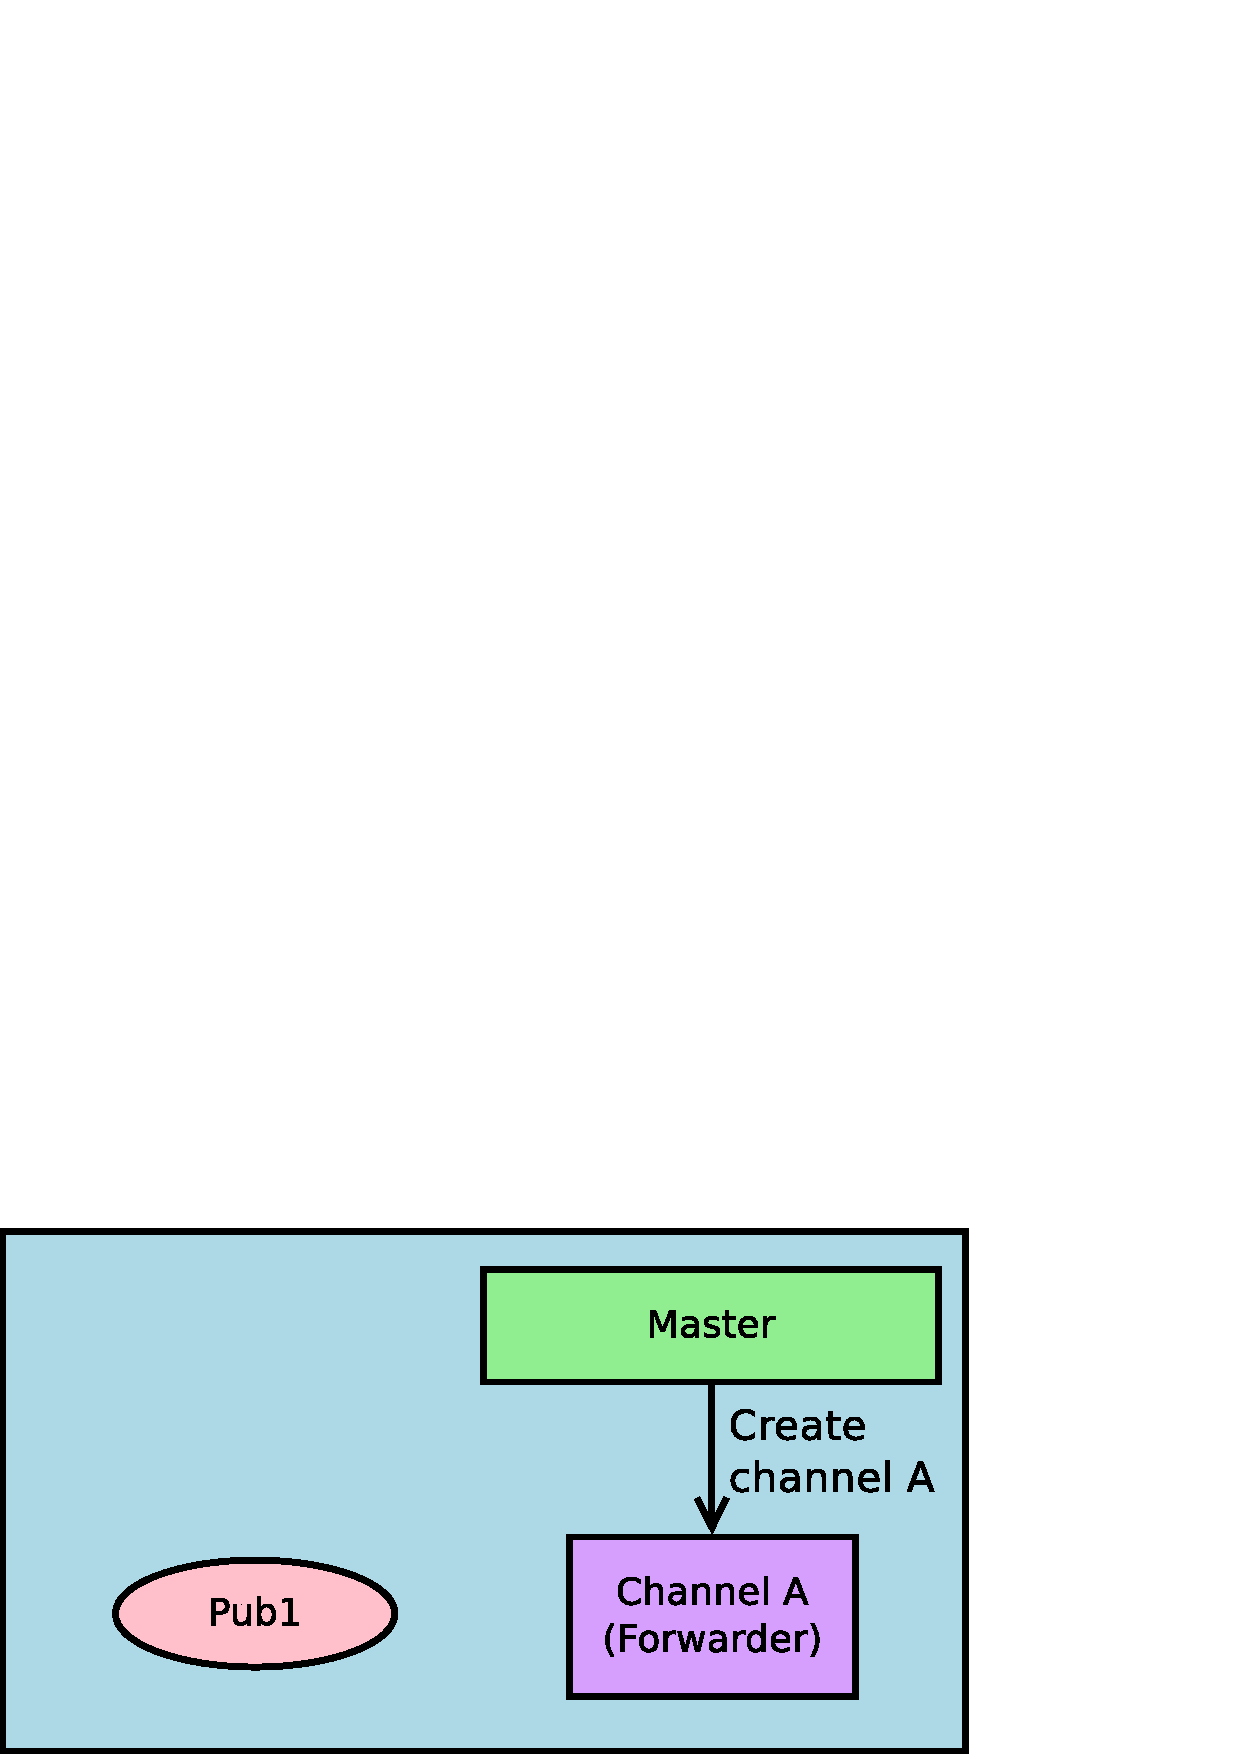
\includegraphics[width=9cm]{./Diagram2.pdf}
\end{center}
\end{frame}


%----------- slide --------------------------------------------------%
\begin{frame}[fragile]
  \frametitle{User Story}
  
The relevant connection credentials are provided by the master to the 
prospective publisher (IP, port, etc for publisher side).
\begin{center}
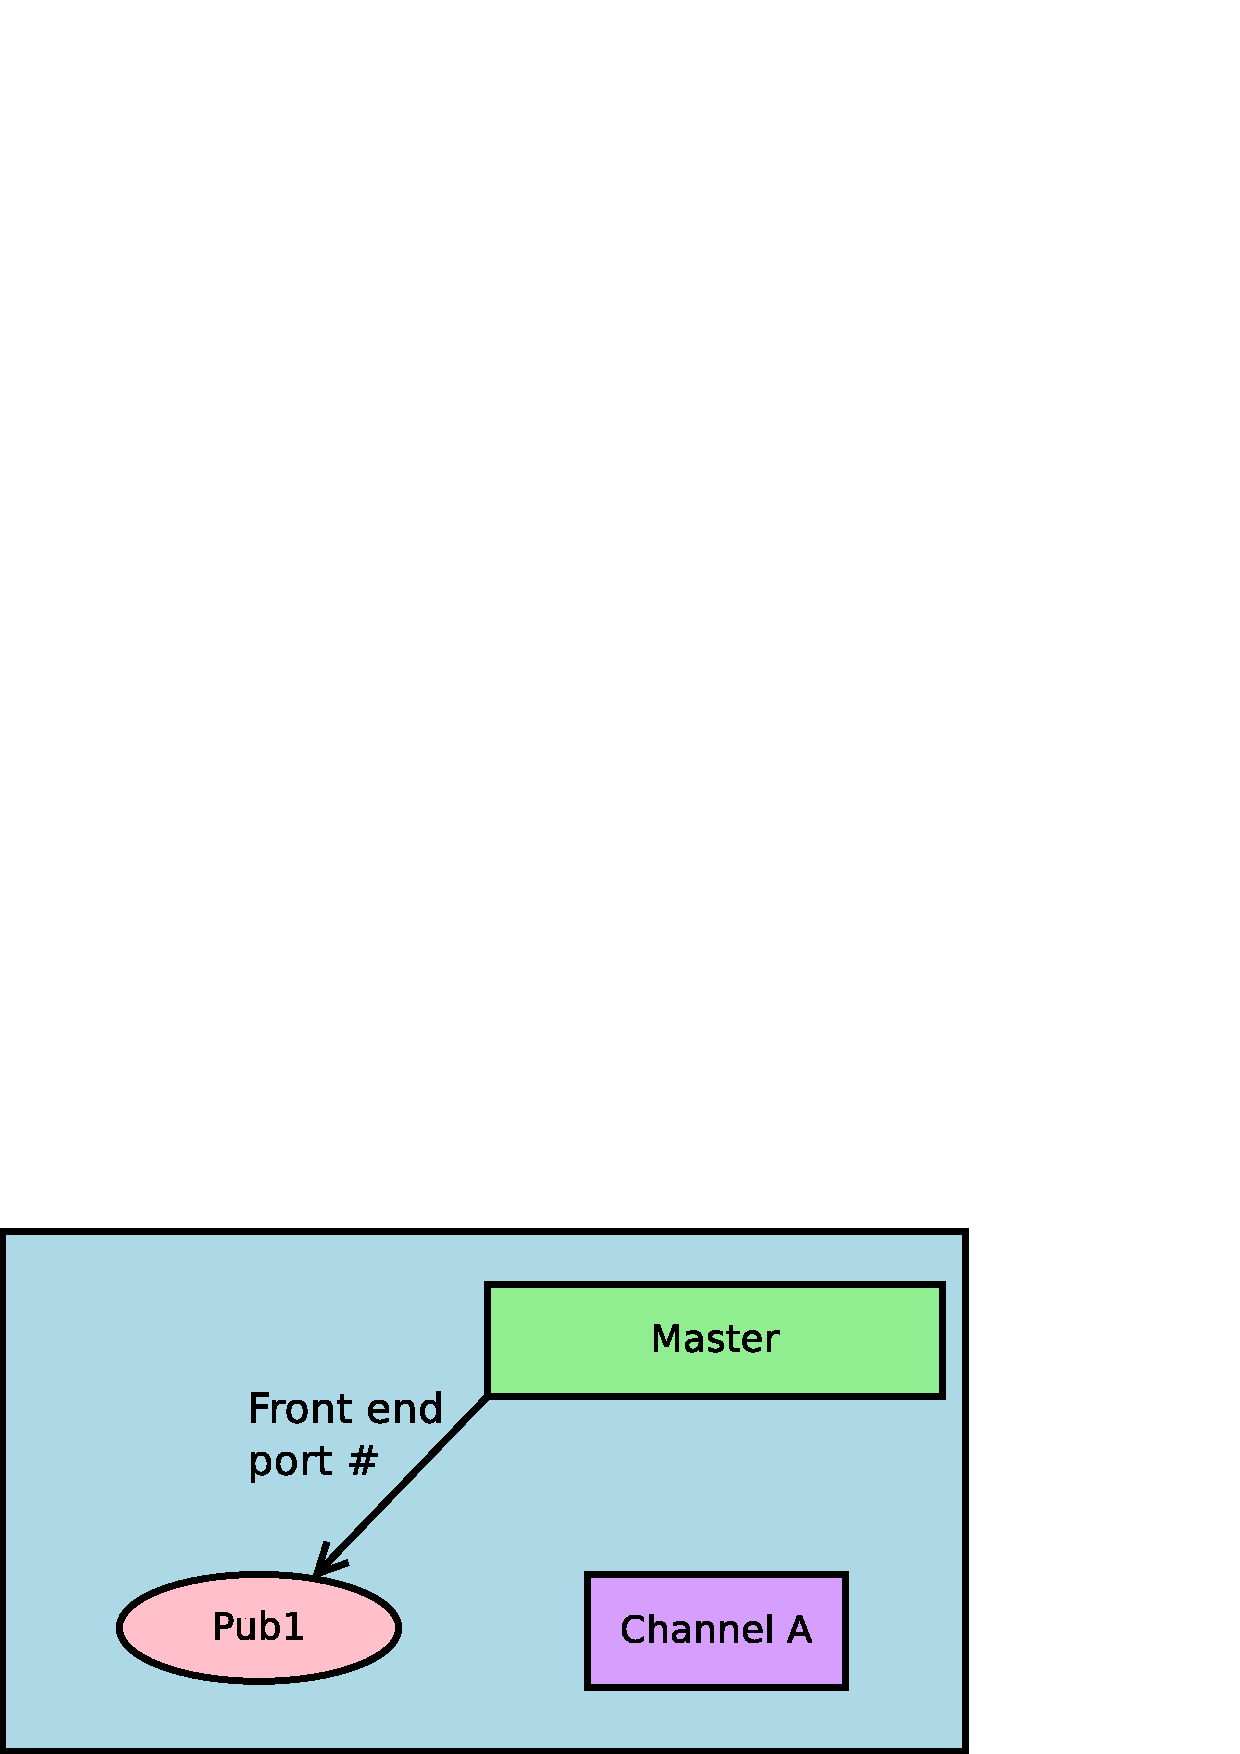
\includegraphics[width=9cm]{./Diagram3.pdf}
\end{center}
\end{frame}


%----------- slide --------------------------------------------------%
\begin{frame}[fragile]
  \frametitle{User Story}
Using the credentials, the process (publisher) can connect with the topic 
``publish'' messages.
\begin{center}
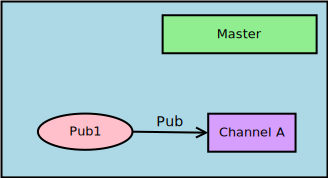
\includegraphics[width=9cm]{./Diagram4.pdf}
\end{center}
\end{frame}


%----------- slide --------------------------------------------------%
\begin{frame}[fragile]
  \frametitle{User Story}
 Another process may enter the process cluster and request to publish 
 on topic A.
\begin{center}
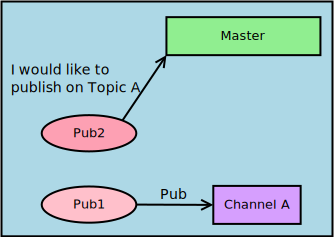
\includegraphics[width=9cm]{./Diagram5.pdf}
\end{center}
\end{frame}


%----------- slide --------------------------------------------------%
\begin{frame}[fragile]
  \frametitle{User Story}
Topic A exists and so the credentials are sent from the Master's database.
\begin{center}
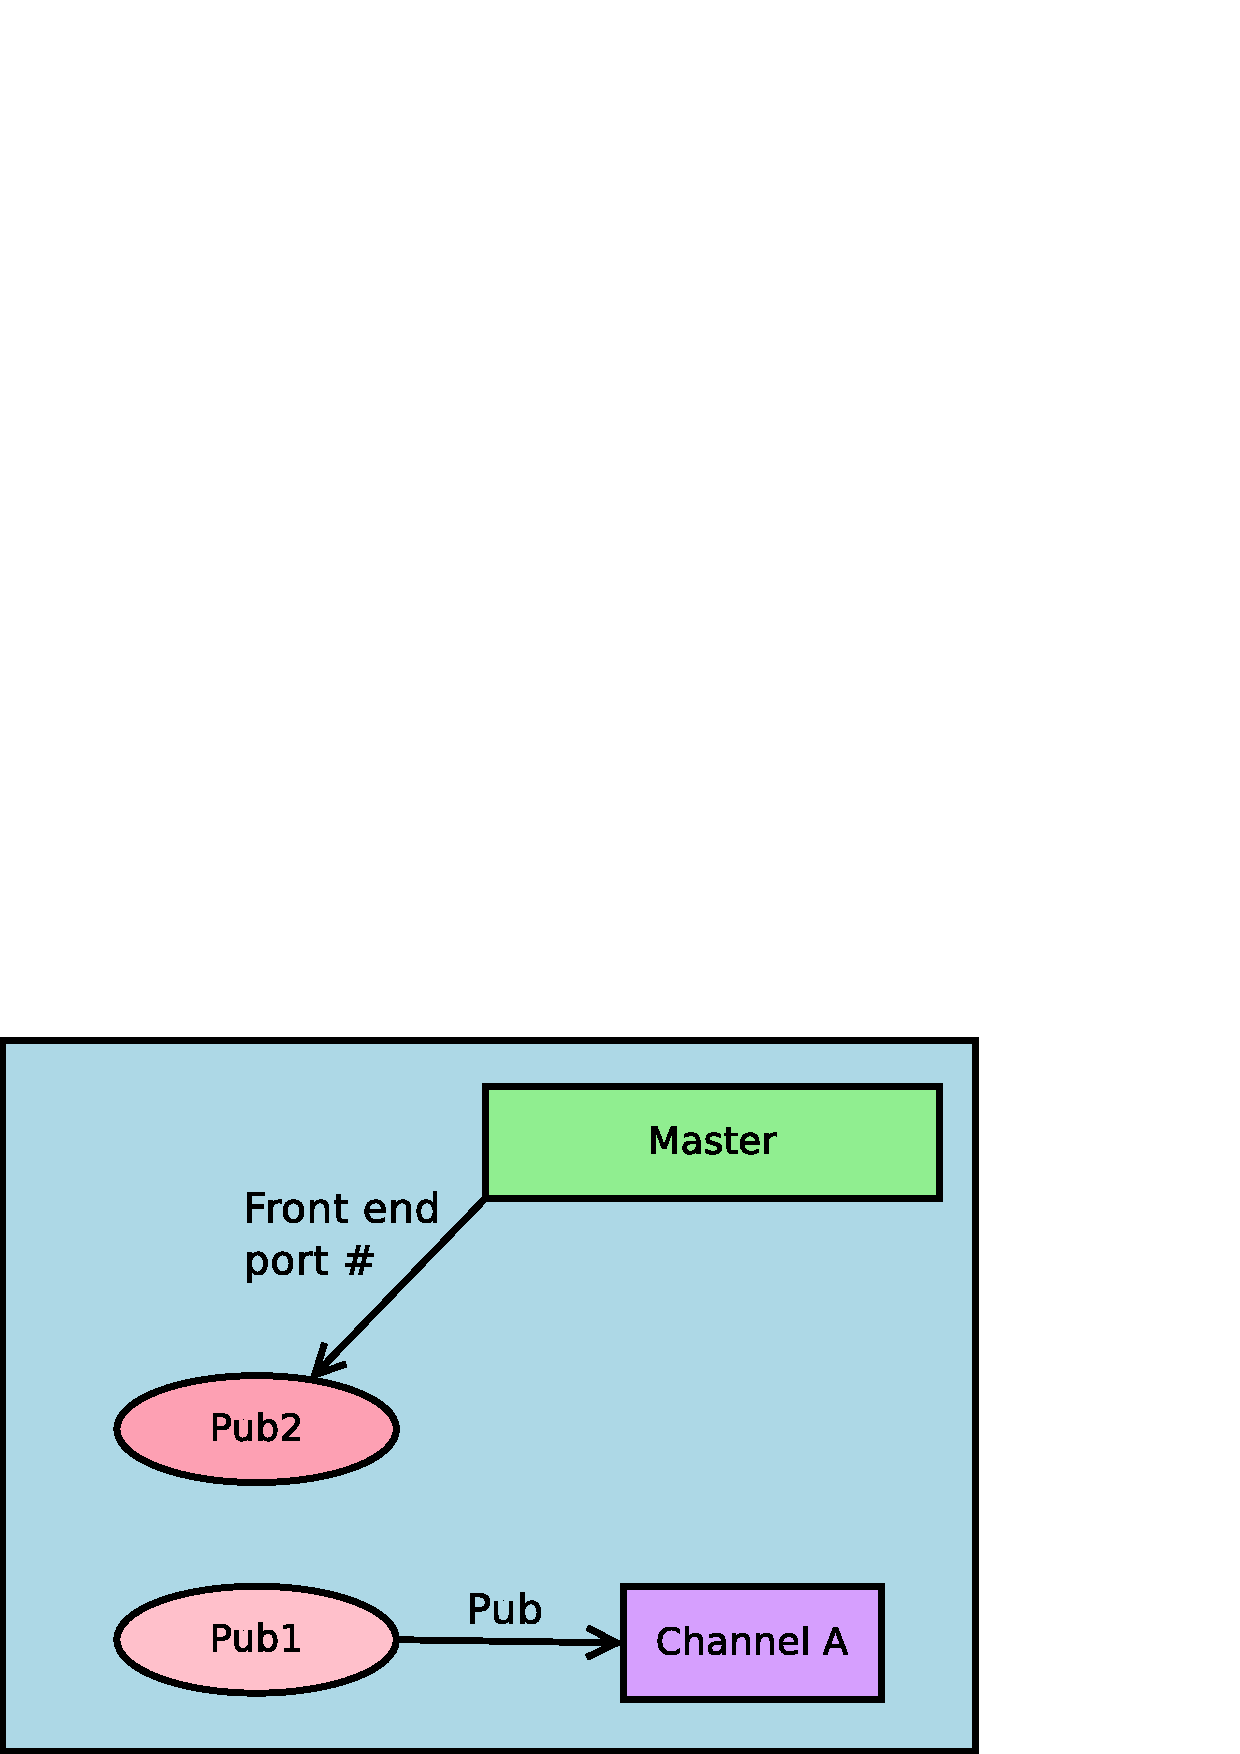
\includegraphics[width=9cm]{./Diagram6.pdf}
\end{center}
\end{frame}


%----------- slide --------------------------------------------------%
\begin{frame}[fragile]
  \frametitle{User Story}
So both processes can publish on the topic.
\begin{center}
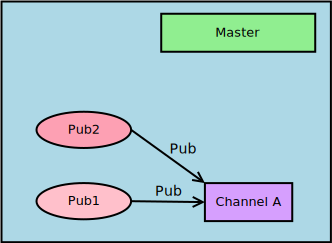
\includegraphics[width=9cm]{./Diagram7.pdf}
\end{center}
\end{frame}


%----------- slide --------------------------------------------------%
\begin{frame}[fragile]
  \frametitle{User Story}
 So far no process is receiving.  Now, another process enters the cluster and
 requests to receive messages from topic A.
\begin{center}
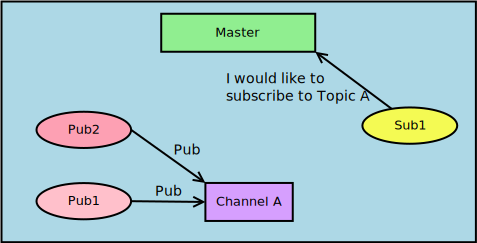
\includegraphics[width=9cm]{./Diagram8.pdf}
\end{center}
\end{frame}


%----------- slide --------------------------------------------------%
\begin{frame}[fragile]
  \frametitle{User Story}
  The master can send the credentials for the receiver side.
\begin{center}
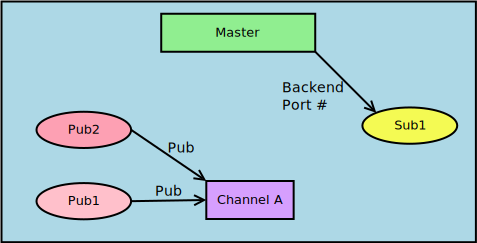
\includegraphics[width=9cm]{./Diagram9.pdf}
\end{center}
\end{frame}


%----------- slide --------------------------------------------------%
\begin{frame}[fragile]
  \frametitle{User Story}
  And this process can connect to the topic and receive the messages.
\begin{center}
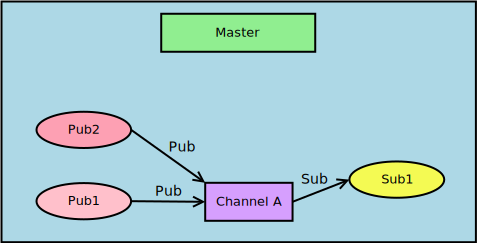
\includegraphics[width=9cm]{./Diagram10.pdf}
\end{center}
\end{frame}


%----------- slide --------------------------------------------------%
\begin{frame}[fragile]
  \frametitle{User Story}
  A fourth process can enter and request to receive messages on topic B.  
  Since this is new, the master will create, store the data in its database.
\begin{center}
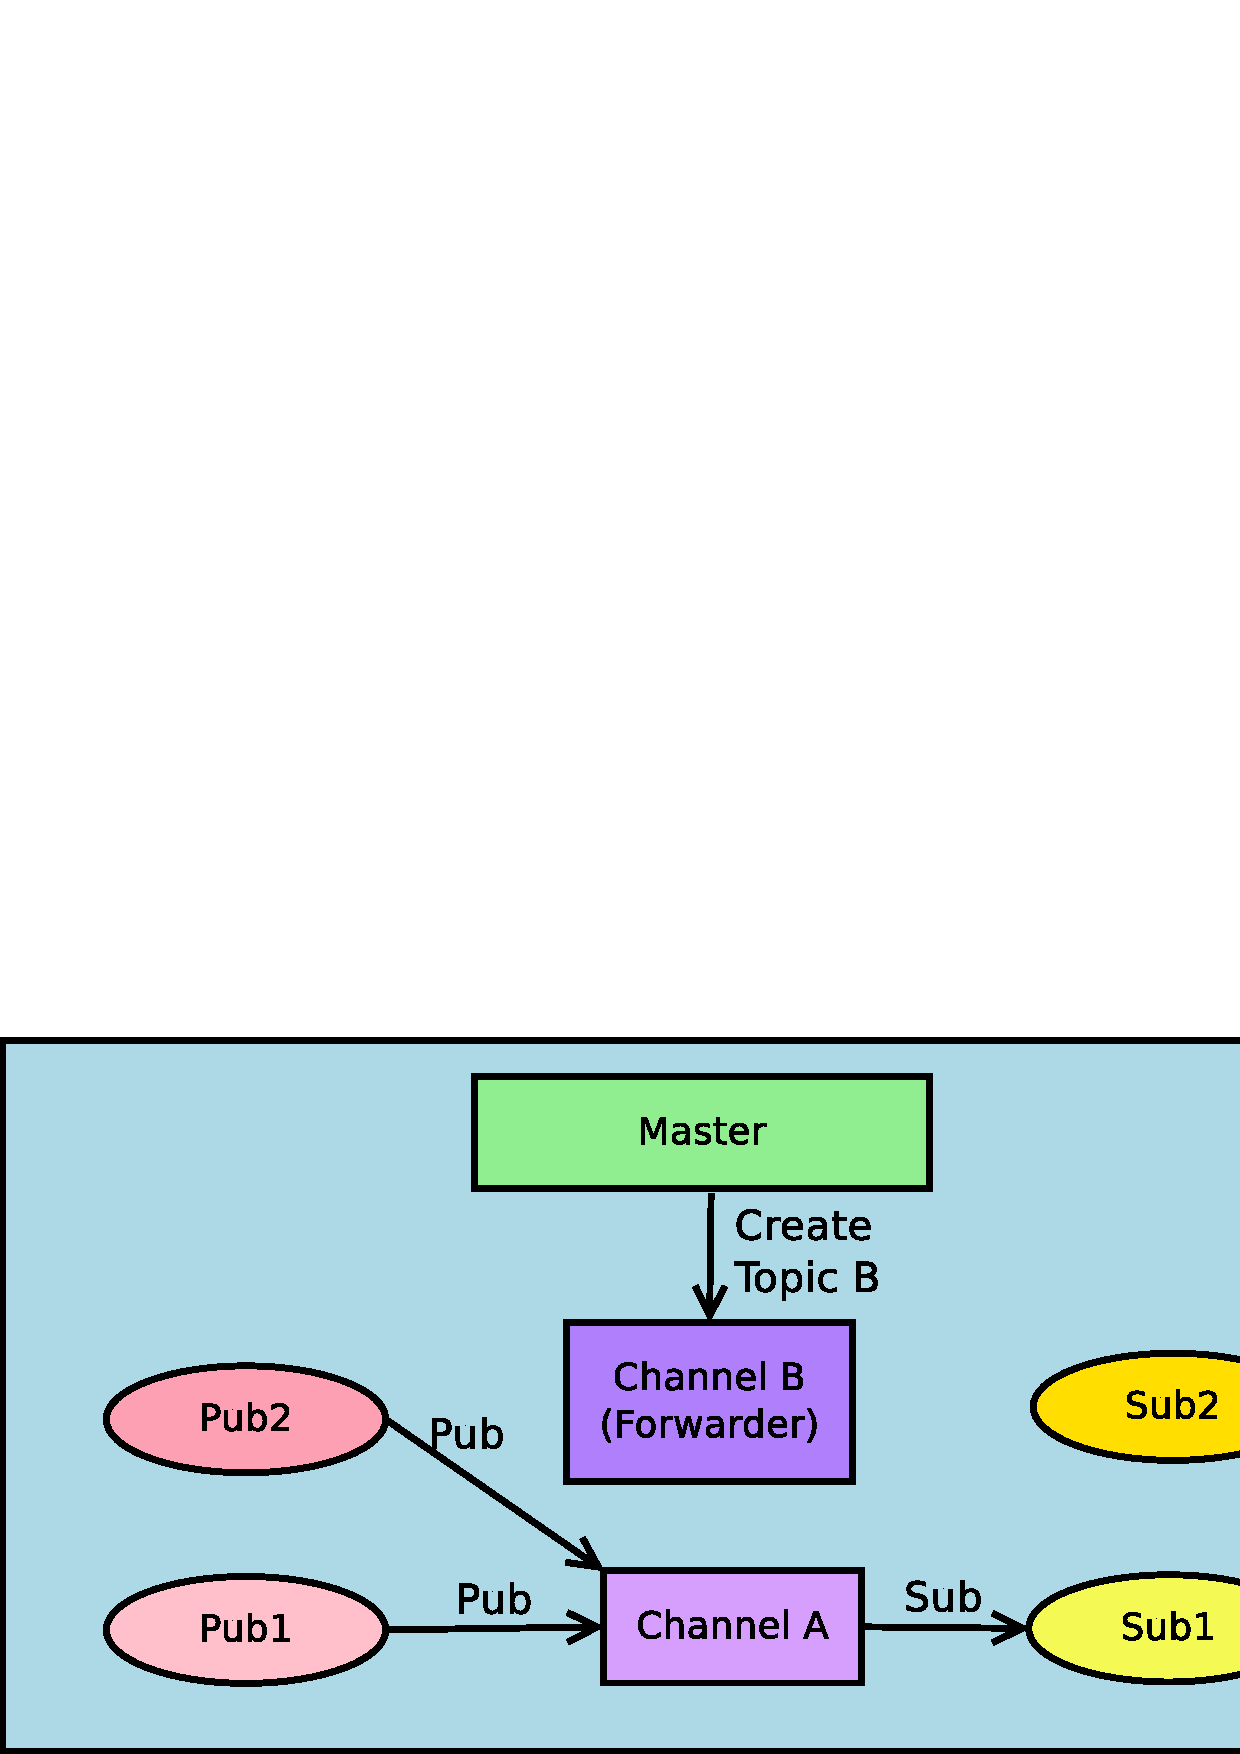
\includegraphics[width=9cm]{./Diagram11.pdf}
\end{center}
\end{frame}



%----------- slide --------------------------------------------------%
\begin{frame}[fragile]
  \frametitle{User Story}
  The master will then provide the relevant credentials to the new 
  subscriber.
\begin{center}
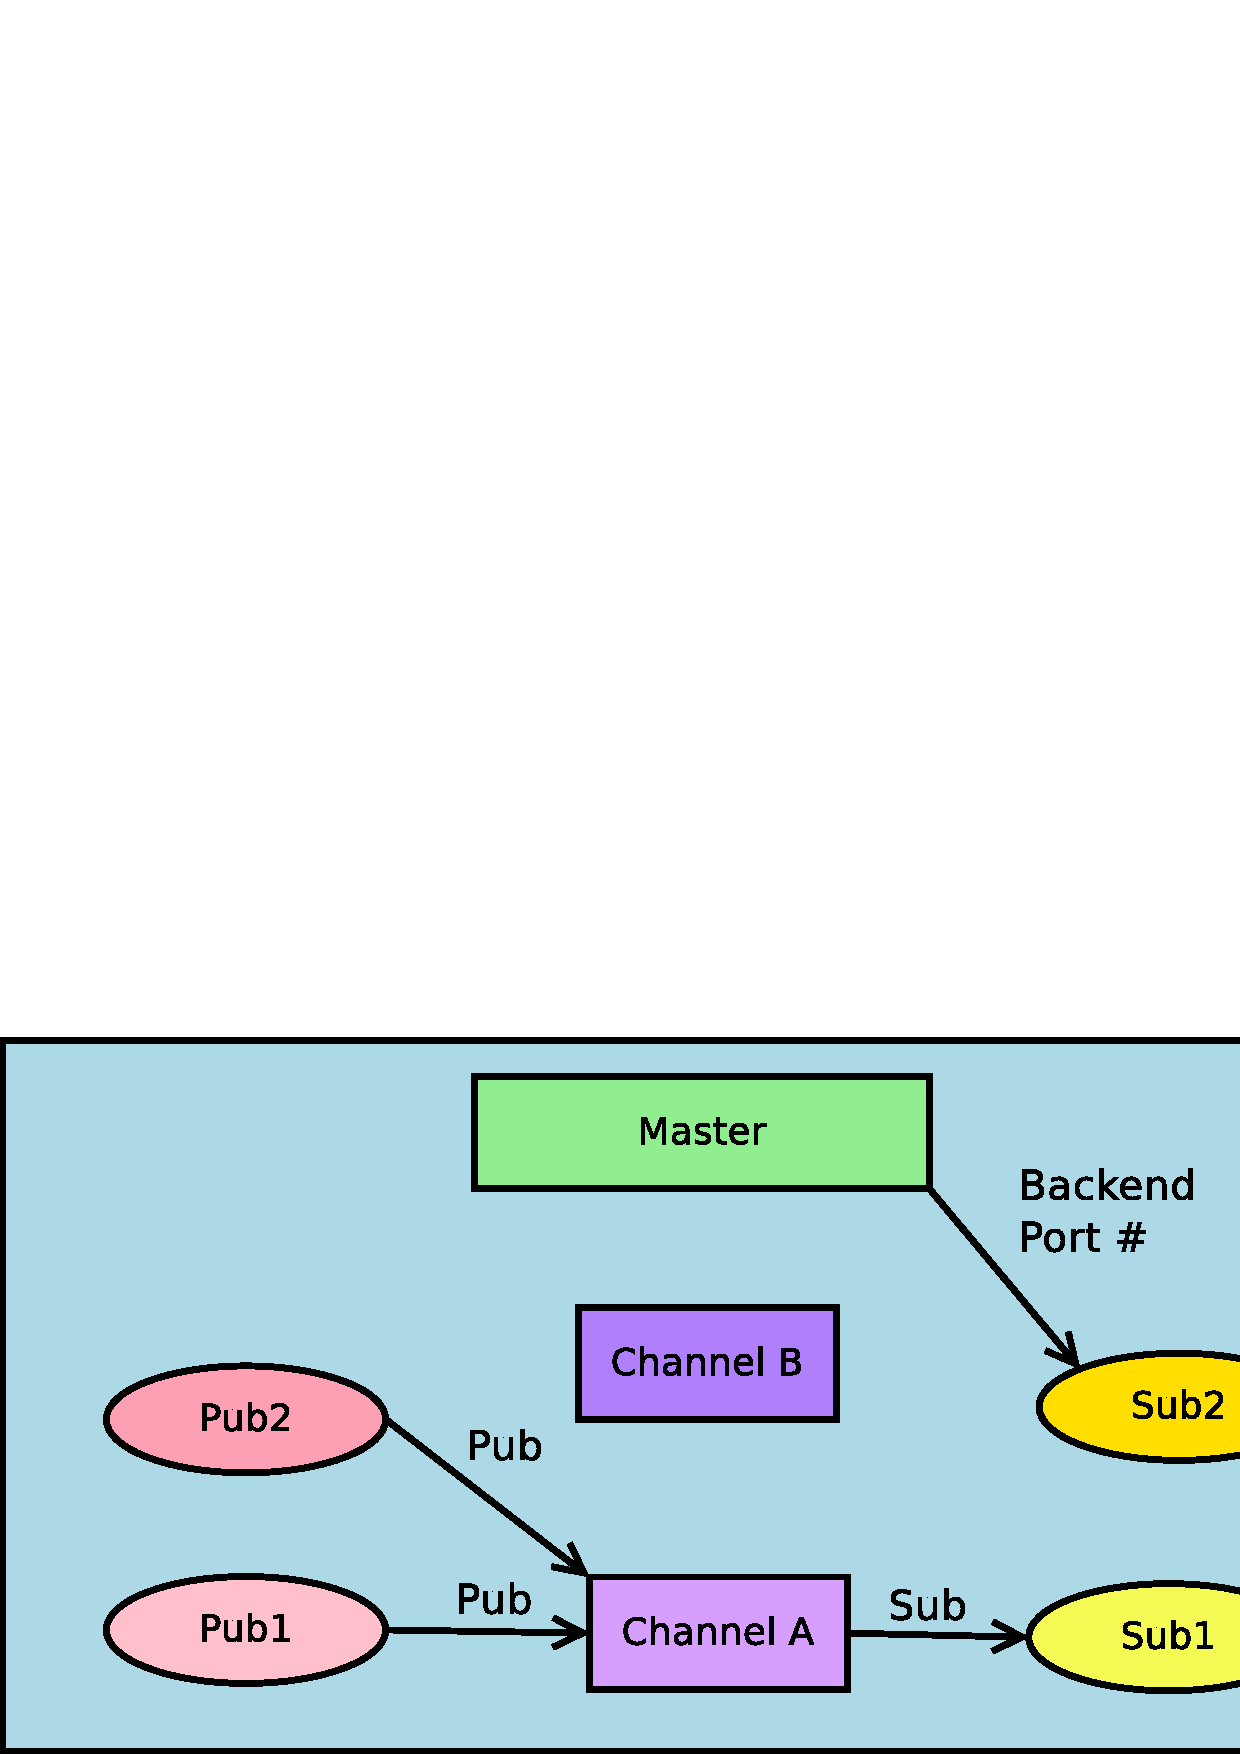
\includegraphics[width=9cm]{./Diagram12.pdf}
\end{center}
\end{frame}




%----------- slide --------------------------------------------------%
\begin{frame}[fragile]
  \frametitle{User Story}
  
  The second subscriber can connect and begin listening.   The point here
 is that it should not matter the order that pubs and subs connect.
\begin{center}
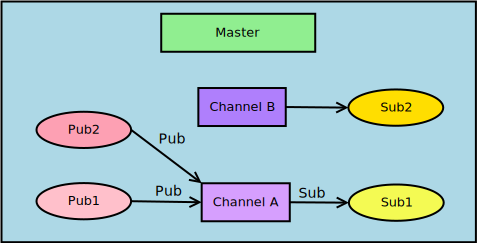
\includegraphics[width=9cm]{./Diagram13.pdf}
\end{center}
\end{frame}



%----------- slide --------------------------------------------------%
\begin{frame}[fragile]
  \frametitle{User Story}
  
A process can publish to multiple topics and can subscribe to multiple 
topics.
\begin{center}
\includegraphics[width=9cm]{./Diagram13b.pdf}
\end{center}
\end{frame}


%----------- slide --------------------------------------------------%
\begin{frame}[fragile]
  \frametitle{More}


The master process is a directory service but not the router or message 
queue.  Messages go directly from process to topic or topic to process.
\vfill


This avoids bottlenecks in scaling.\vfill

Master keeps database of ports and IPs all pubs and sub.   Keeps 
ports and IPs for processes managing the topics.


\end{frame}


%----------- slide --------------------------------------------------%
\begin{frame}[fragile]
  \frametitle{Master}
\begin{center}
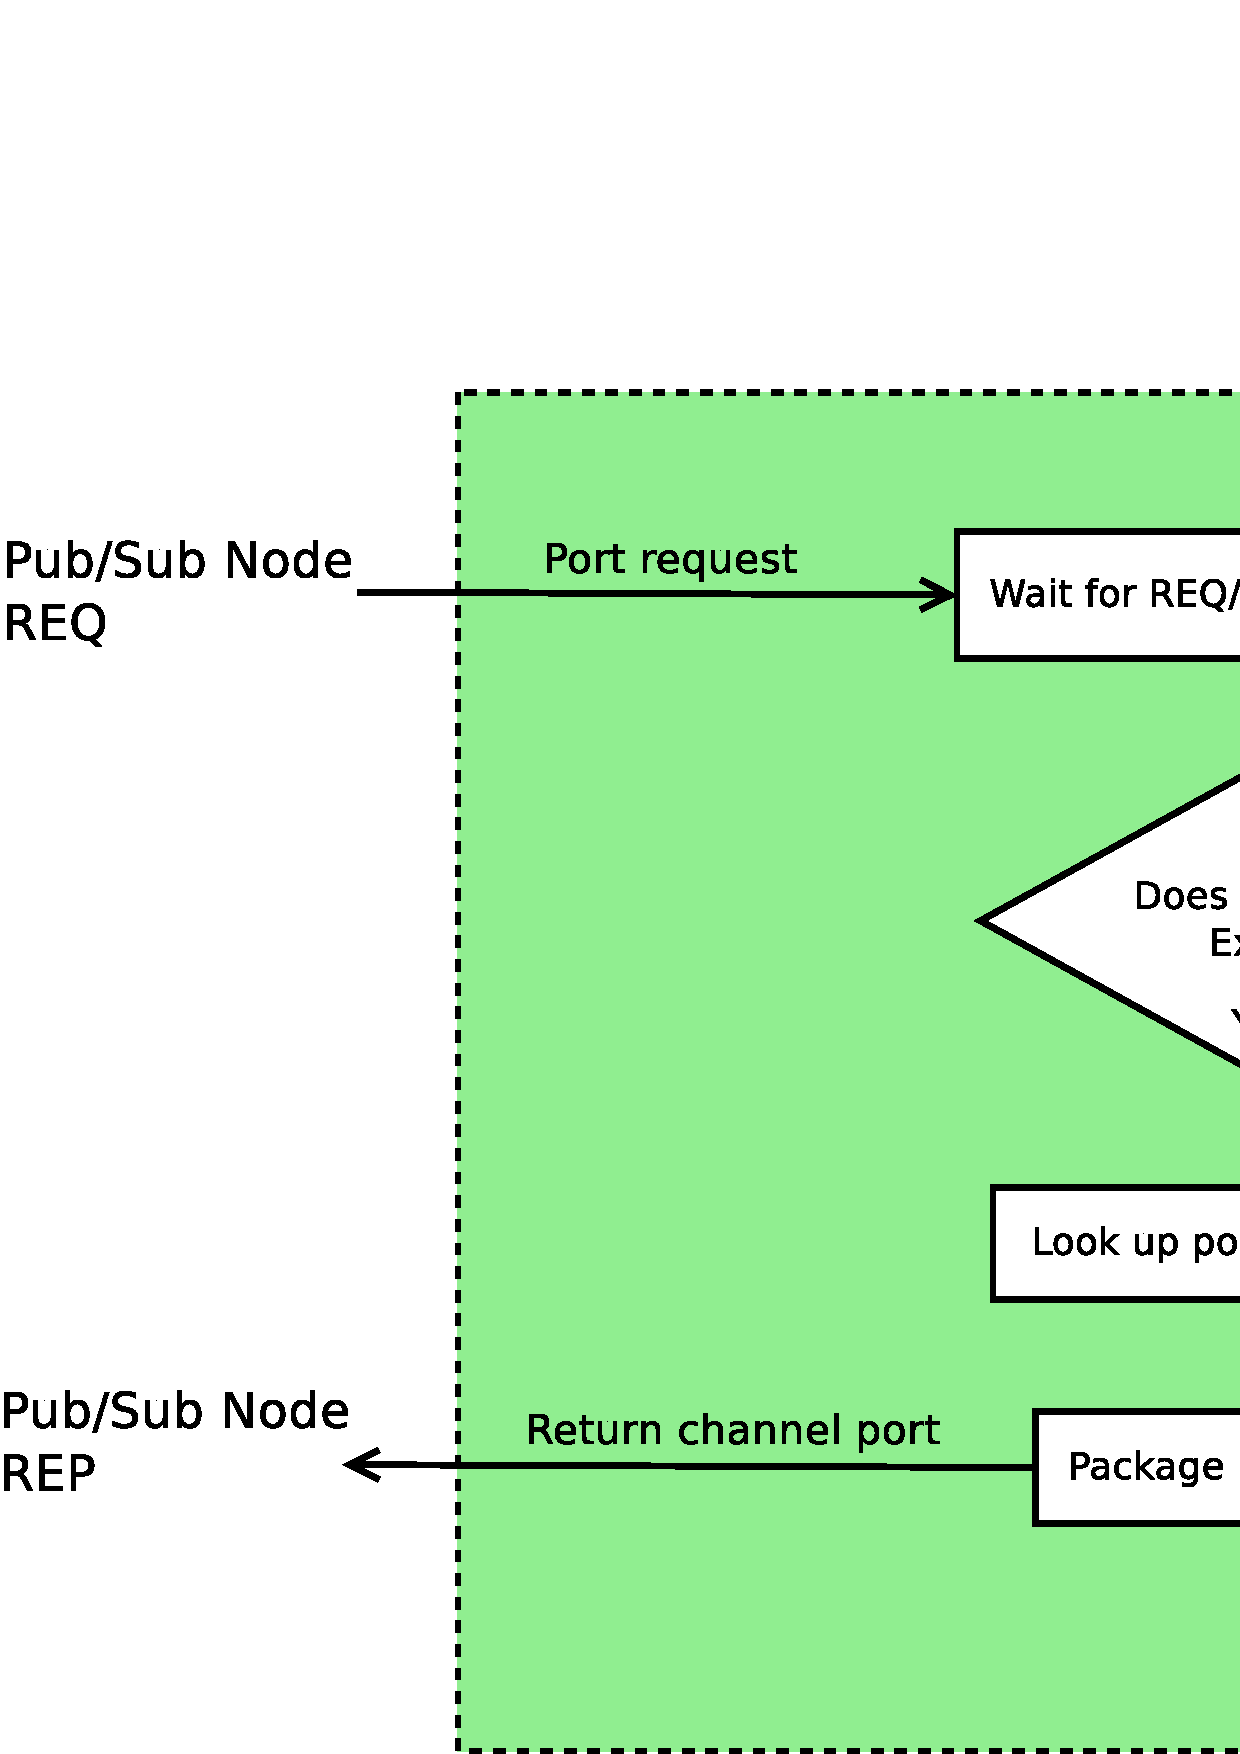
\includegraphics[width=12cm]{./Diagram14.pdf}
\end{center}
\end{frame}



%----------- slide --------------------------------------------------%
\begin{frame}[fragile]
  \frametitle{Python Code Concept - Publisher}
\begin{verbatim}
import tala as tl

master = "default"
name = "talkernode"
tl.join(name,master)

topic = "realityTV"

pub = tl.publisher(topic)

key = "0"
message = tl.pack("It is all scripted.")
tl.send(pub, message, key)

\end{verbatim}
\end{frame}



%----------- slide --------------------------------------------------%
\begin{frame}[fragile]
  \frametitle{Python Code Concept - Subscriber}
\begin{verbatim}
import tala as tl

master = "default"
name = "listennode"
tl.join(name,master)

topic = "realityTV"

sub = tl.subscribe(topic)

flag = 0  # timeout codes
message, key = tl.receive(sub, flag)
print(tl.unpack(message))

\end{verbatim}
\end{frame}


%----------- slide --------------------------------------------------%

\begin{frame}[fragile]
  \frametitle{Aspects}

There are configuration aspects (in a config file and dynamic).
\begin{itemize}
\item Message queue size.
\item Message removal behavior and if multiple buffers required.
\item Full FIFO behavior.
\item Message data types.
\item Message data marshalling.
\end{itemize}

\end{frame}


%----------- slide --------------------------------------------------%

\begin{frame}[fragile]
  \frametitle{Alternate Design}

The topic can be bound to the subscriber.
\vfill

The master will hand the subscriber's IP/port to the publisher and point to point communciation would happen. \vfill

   For multiple subscribers, the master would need to contact each publisher and add a subscriber to their broadcast list.\vfill
   
Much of the user stories are the same, just the change in the location of the FIFO.

\end{frame}


%----------- slide --------------------------------------------------%
\begin{frame}[fragile]
  \frametitle{Alt Design}
\begin{center}
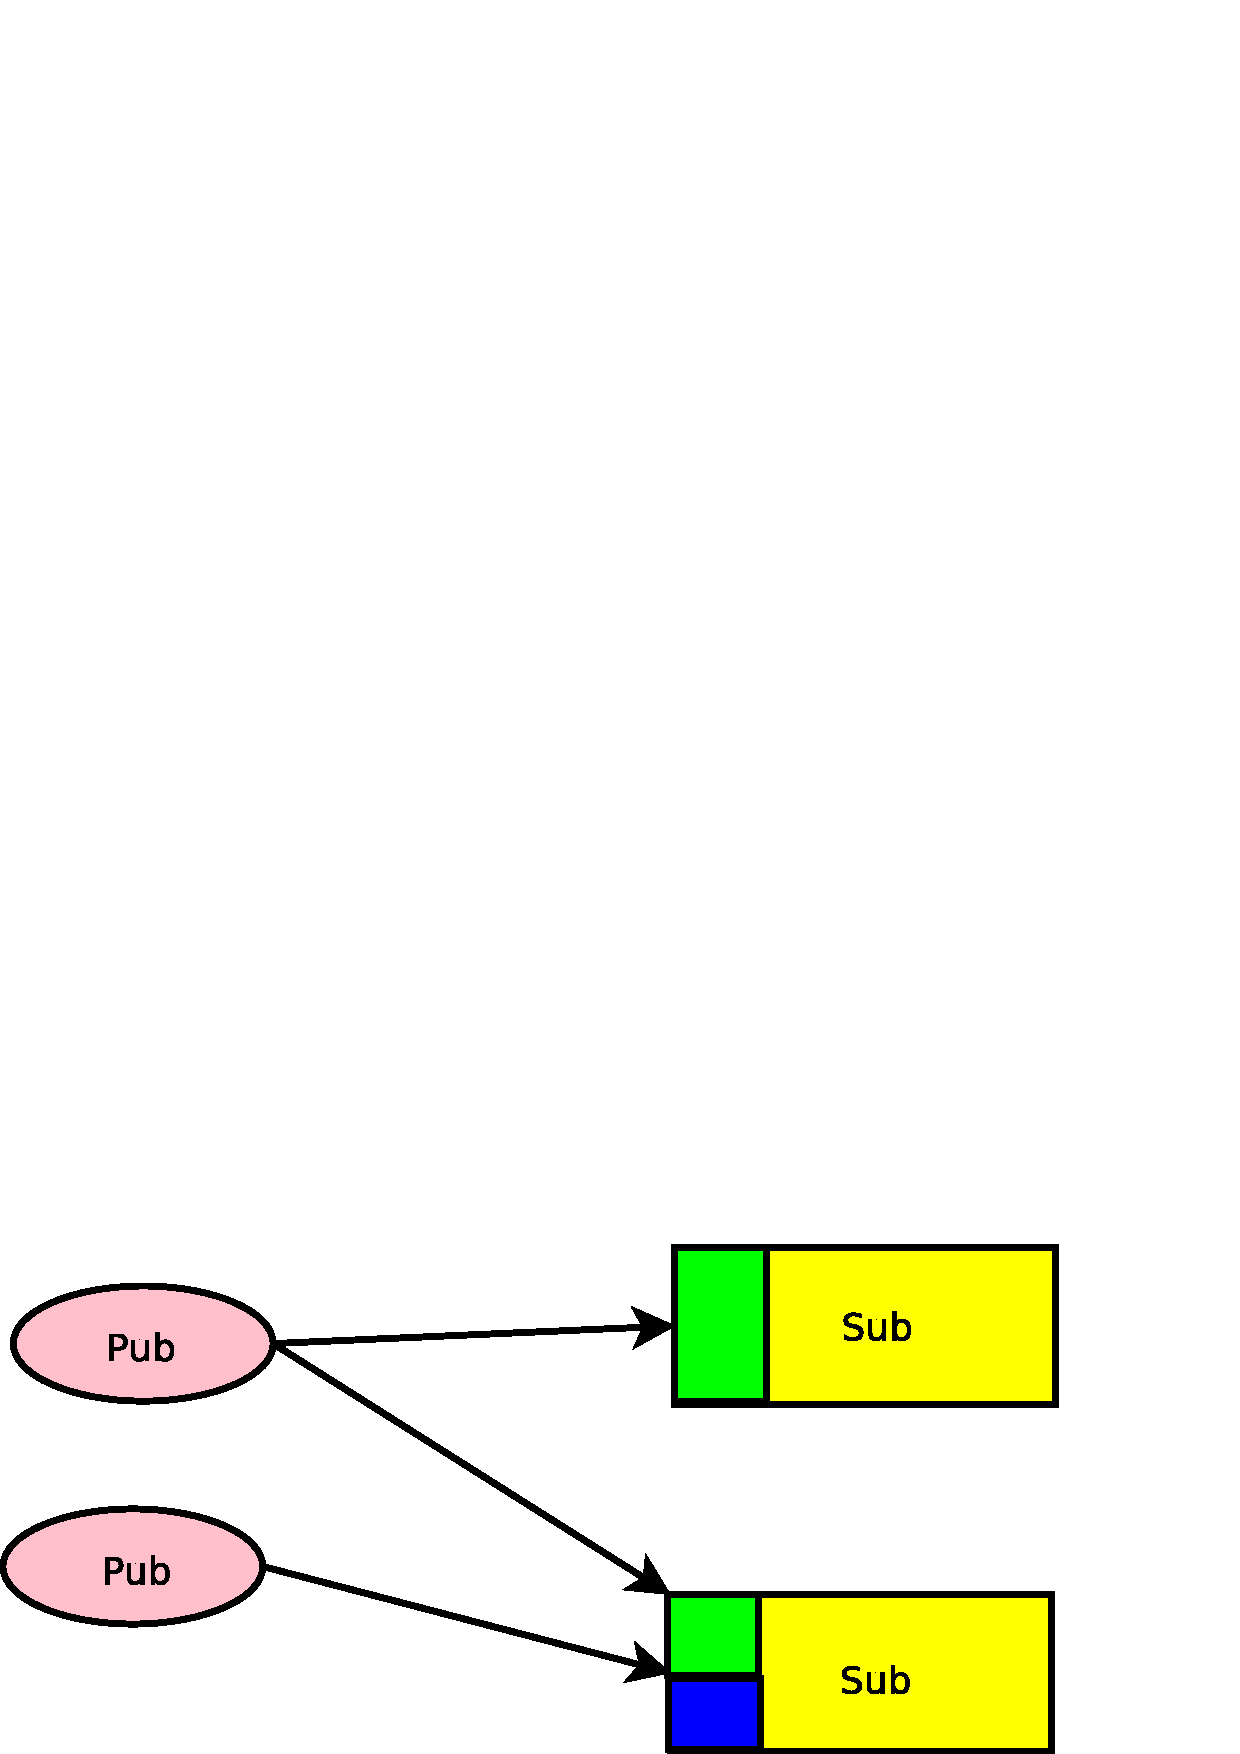
\includegraphics[width=10cm]{./Diagram15.pdf}
\end{center}
\end{frame}




%----------- slide --------------------------------------------------%
\begin{frame}[fragile]
  \frametitle{Design Issues}

\begin{itemize}
\item Binding languages:  Julia, Python, Rust
\item Language for master (Rust or C++)
\item Threading architecture
\item Communication lib (0MQ vs Sockets)
\item Communication architecture
\item FIFO architecture
\end{itemize}

\end{frame}


%----------- slide --------------------------------------------------%
\begin{frame}[fragile]
  \frametitle{Tools etc}

\begin{itemize}
\item GUI management tool
\item Node/topic Graph plotting tool
\item Listener and Talker examples in various languages.
\end{itemize}
\vfill

Open source aspects (host, license, etc)

\end{frame}



%----------- slide --------------------------------------------------%
\begin{frame}[fragile]
  \frametitle{Requirements}

\begin{itemize}
\item Directory service 
\begin{itemize}
\item  Separate process
\item  Tracks nodes in the compute cluster
\item  Answers requests for node communication data
\item  Internal database for network graph
\item  API for GUI management
\end{itemize}
\item Python \& Julia APIs
\begin{itemize}
\item Node registration 
\item Pub/sub/req/rep setup functions
\item Push/pop/send/receive functions
\item Node exit and admin functions
\end{itemize}
\item GUI Management
\begin{itemize}
\item  Launch master
\item  Runtime config
\item  Port ranges
\end{itemize}
\item Graph tool
\begin{itemize}
\item Present the node-topic graph
\end{itemize}
\end{itemize}


\end{frame}





%----------- slide --------------------------------------------------%
\begin{frame}[fragile]
  \frametitle{Software Expectations}

\begin{itemize}
\item A prototype of the directory service - aka master.
\item An initial API module for Python and Julia for calling Tala.
\item A prototype of the GUI management tool.
\item A prototype of the network graph tool.
\item Some sample programs to illustrate Tala.
\end{itemize}


\end{frame}


%----------- slide --------------------------------------------------%
\begin{frame}[fragile]
  \frametitle{Project Expectations}

\begin{itemize}
\item Design - because this is Senior Design.
\item Communication - keep a dialog.\footnote{I can handle bad news - I don't want any surprises}
\item Teamwork - a sense of service to others.
\item A great attitude - because every day is a gift.
\item Open source project - with software described above.
\item Documentation - of the code and the experience.
\end{itemize}

\end{frame}


\end{document}

